%%%%%%%%%%%%%%%%%%%%%%%%%%%%%%%%%%%%%%%%%%%%%%%%%%%
% ioni.tex
%%%%%%%%%%%%%%%%%%%%%%%%%%%%%%%%%%%%%%%%%%%%%%%%%%%

\Gfour{} offers a range of ionization models for different particle types.  These 
models can be classified as either condensed or discrete.  In the condensed 
approach, the energy loss calculation has a continuous component and a discrete
one, discriminated by a given energy threshold.  Below this threshold the energy
loss is continuous, and above it the energy loss is simulated by the explicit 
production of secondary electrons \cite{embib:design}.  The user does not 
directly define the threshold because in \Gfour{} a special method of threshold 
calculations for different materials is used.  The user defines a unique 
\emph{cut in range}  \cite{bib:G4}, whose value is transformed into a kinetic 
energy threshold per material at initialization time of \Gfour{}.  Electrons 
with this kinetic energy have a mean range in a given material equal to the cut
in range and gammas have an absorption length 1/5 of the range cut.

If no value is given in the reference physics lists the default cut value of 
0.7 mm is used, providing sufficiently accurate simulation results for many 
applications.  For a specific use-case, \emph{cut in range} values should be 
optimized per geometry region.  It is recommended that this value be defined to
be less than the smallest size of geometry volumes in the region.
 
The \emph{cut in range} approach may be used for other processes besides 
ionization.  These cuts may be defined for gammas, electrons, positrons, and 
protons, and modified based on particle type and geometry region.  However, the
cut value cannot be arbitrary.  Because \Gfour{} ionization models usually have an
energy range of applicability, there is a lower limit to the electron production 
threshold.  By default the lower limit is 1 keV, but it can be changed by the 
user.  On top of this, any EM model may establish its own lower limit for the 
threshold.  If several models are applied for a given particle type, then the 
maximum of all limit values from the models is used for the particle.  For most 
ionization models the low limit is equal to the mean ionization potential of a
material. 

The list of main ionization processes and models following the condensed 
simulation approach is shown 
in Table \ref{Table-Ioni}. 
\begin{table*}
\caption{List of \Gfour{} ionization processes and models with recommended energy range.}
\label{Table-Ioni}
\begin{center}
\begin{tabular}{llll}
\hline
Particle& Process& Model& Energy range\\ \hline
 e-/e+& \gclass{G4eIonisation} & \gclass{G4MollerBhabhaModel} & 10 keV - 10 TeV\\
 e-/e+ & & \gclass{G4PenelopeIonisationModel} & 0.1 keV - 5 GeV\\
e- &  & \gclass{G4LivermoreIonisationModel} & 0.1 keV - 1 MeV \\
all & & \gclass{G4PAIModel} &   0.1 keV -  10 TeV  \\
all & & \gclass{G4PAIPhotModel} & 0.1 keV -  10 TeV \\
muons & \gclass{G4MuIonisation} & \gclass{G4BraggModel} & 0.1 keV -  0.2 MeV \\
& & \gclass{G4BetheBlochModel} & 0.2 MeV -  1 GeV \\
& & \gclass{G4MuBetheBlochModel} \cite{embib:emmu}& 1 GeV -  10 PeV \\ 
hadrons& \gclass{G4hIonisation} & \gclass{G4BraggModel} & 1 keV -  2 MeV\\
& & \gclass{G4BetheBlochModel} & 2 MeV -  10 TeV \\
& & \gclass{G4ICRU73QOModel} \cite{embib:empbar} &  5 keV -  10 MeV \\
ions & \gclass{G4ionIonisation} & \gclass{G4BraggIonModel} & (1 keV - 2 MeV)/u \\
& & \gclass{G4BetheBlochModel} & (2 MeV -  10 TeV)/u \\
 & & \gclass{G4IonParametrisedLossModel} \cite{embib:emIon}&  (1 keV - 1 GeV)/u \\
\hline
\end{tabular}
\end{center}
\end{table*}

In the condensed approach, a model of energy loss fluctuations must be used in
conjunction with the energy loss model.  The \gclass{G4VEmFluctuationModel} 
interface was developed to accommodate several implementations of fluctuation
sampling, and several models derive from it:
\begin{itemize}
\item \gclass{G4UniversalFluctuation} - default model applicable to all charged 
particles based on a previous model \cite{embib:fluc};
\item \gclass{G4IonFluctuations} -  for small steps uses
\gclass{G4UniversalFluctuation} and for big steps uses a gaussian width based
on a parameterization \cite{embib:ionfluc};
\item \gclass{G4PAIModel} and \gclass{G4PAIPhotModel} - photo-absorption 
ionization (PAI) models \cite{embib:pai}.
\end{itemize}
PAI models simultaneously provide cross sections and energy loss, and sample
energy loss fluctuations.  The ionization cross sections of the PAI models
derive from gamma absorption cross sections per atomic shell.  They are, in 
general, more accurate and stable versus simulation conditions (cuts, step 
limits, energy) than the default model \cite{embib:chep14,embib:chep11}, but are
more computationally expensive because of the internal sampling at each
ionization collision.  An illustration of simulation performance is shown in 
Figure~\ref{em:alice} for the test beam data of the ALICE Time Projection 
Chamber \cite{embib:tpc1,embib:tpc2}. 

Other studies show that PAI models generally fit the data 
independently of the step size, while the default model strongly requires the
application of extra step limitations. 

In the case of thin absorbers, the default model requires at least two particle
steps within the defined volume.  While having some difficulties for thin 
layers, the default model provides good physics performance for a variety of 
applications, in particular for tracking devices (Figure~\ref{em:silicon}), 
satisfying the requirements of most HEP experiments.

\begin{figure}
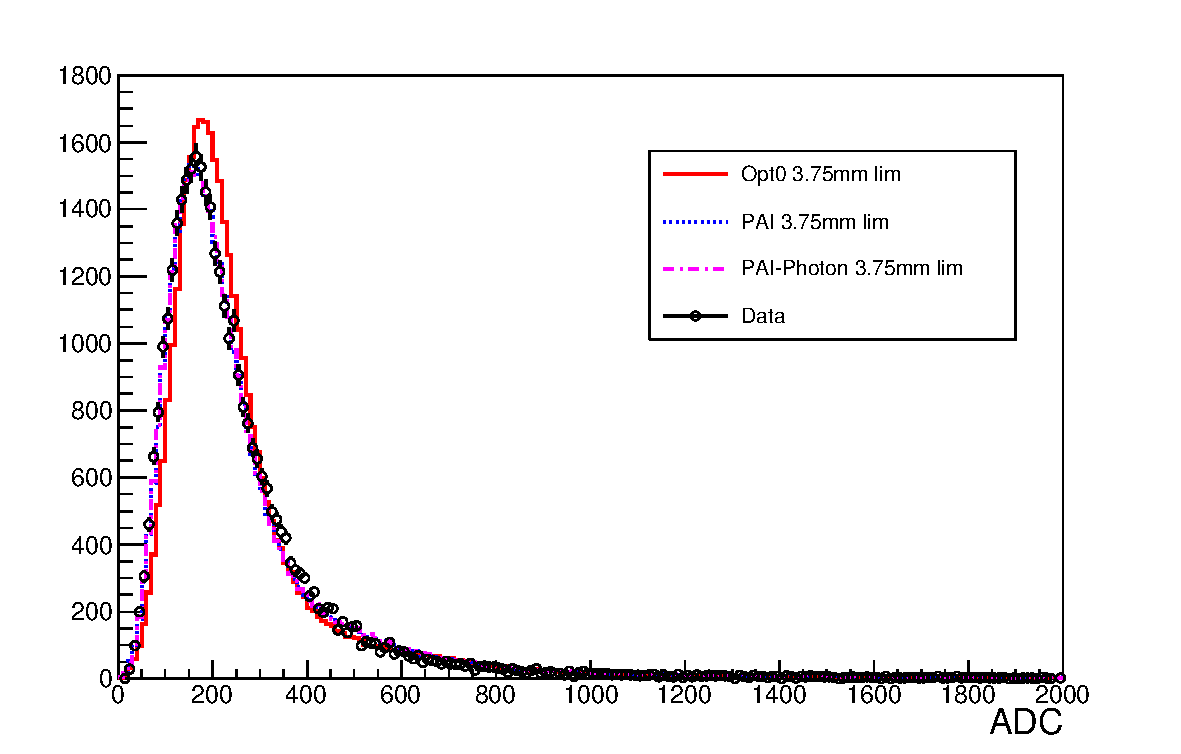
\includegraphics[width=0.5\textwidth]{figures/A_p_3gev_1mm.pdf}
\caption{Proton energy deposition in gas gap in ADC counts for a beam momentum 
         of 3 GeV/c and a gas mixture of $Ne-CO_2-N_2$.  
         The histogram represents the simulation with a 1 mm cut and a step limit
         equal to half the gap thickness.  The ADC scale for simulation was 
         normalized to the PAI model peak position.  The open circles display
         the data \cite{embib:tpc1,embib:tpc2}.}
\label{em:alice}
\end{figure}

\begin{figure}
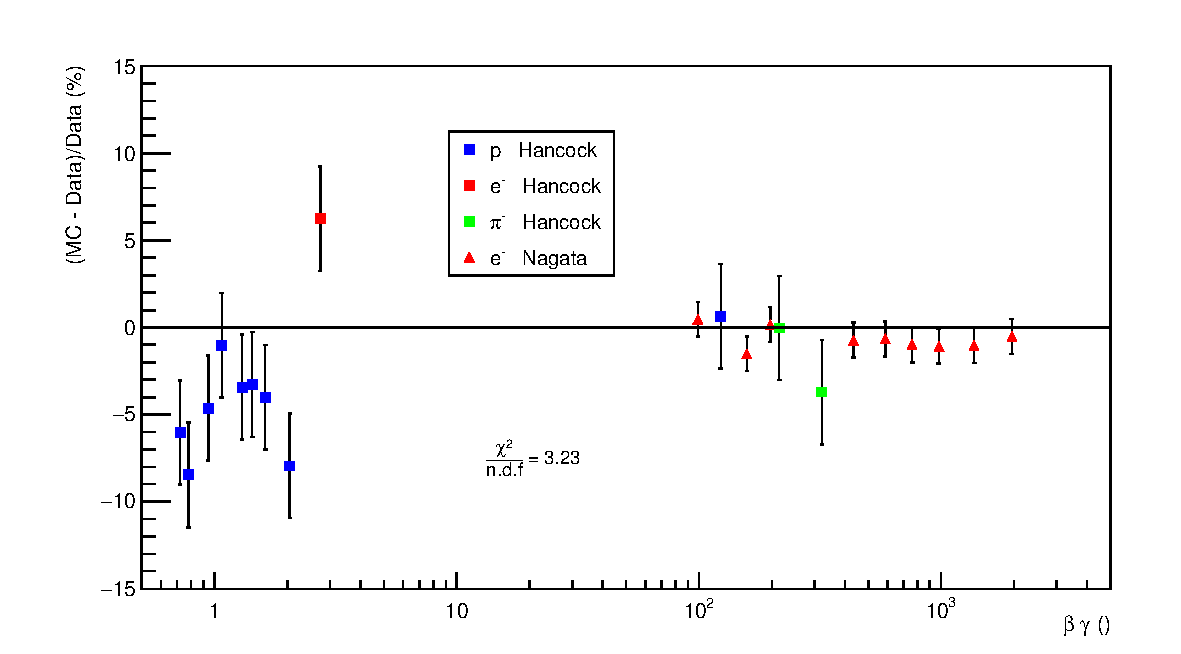
\includegraphics[width=0.5\textwidth]{figures/BetaGamma_Delta_diff_opt0_10um.pdf}
\caption{\Gfour{} versus data comparison of the most probable energy deposition in 
         thin layers of silicon (thickness 300 $\mu m$ Hancock; 1565 $\mu m$ Nagata). 
         Different beam particles and energies are used from the review
         \cite{embib:bicsel}.  Results are given in percent, and the default EM 
         physics is applied with a cut in range of 100 $\mu m$.}
\label{em:silicon}
\end{figure}

\begin{figure}
% \centering
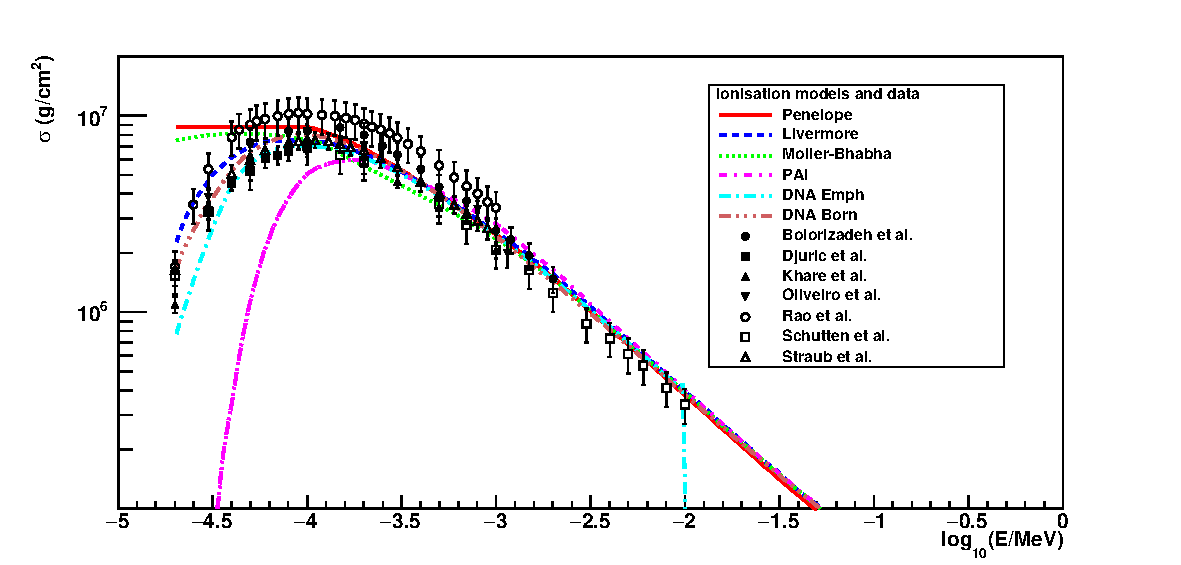
\includegraphics[width=3.8in]{figures/ApicXS_99.pdf}
\caption{Total cross section of delta electron production in liquid water as a
         function of projectile electron energy.  Curves correspond to different
         \Gfour{} ionization models, and points correspond to experimental data
         \cite{embib:dnaxs}.  The DNA model has an upper validity limit of
         1 MeV.}
\label{em:xsh2o}
\end{figure}

Recently, alternative ionization processes and models were introduced for
specific applications.  Contrary to the traditional condensed approach, these 
processes do not have a continuous energy loss component.  They explicitly 
generate all electrons down to very low energies.  They were first developed in
the framework of the \Gfour{}-DNA project (see \ref{sec:em9}), which aims to model
early biological damage induced by ionizing radiation at the DNA scale.  The 
\gclass{G4DNAIonisation} process has different models that apply to electrons, 
protons and selected ions (H, alpha, alpha+, He, Li, Be, B, C, N, O, Si and Fe)
in liquid water \cite{embib:dnaProc1, embib:dnaxs}.  Similarly, a specific
process, \gclass{G4MicroElecInelastic}, was developed for microelectronics 
applications, with a corresponding model that applies to electrons, protons and
heavy ions in silicon \cite{embib:micro, embib:micro1}.

Such models are applicable to a limited energy range and a selected set of 
materials, and in order to simulate realistic particle transport, it may be 
necessary to combine them with a continuous ionization process.  For this 
purpose the user may configure, for a given process and particle type,
several models for different energy ranges and detector regions \cite{bib:uni}.
These discrete models produce secondary electrons without the low energy 
threshold used by continuous ionization models, which could lead to 
discontinuous transitions between models.  To remedy this, the production of 
secondary electrons below the threshold may be enabled using the 
\gclass{G4VSubCutProsessor} interface, which works in parallel with the 
continuous model.

To illustrate this, cross sections of electrons in liquid water are shown in
Figure \ref{em:xsh2o}.  For the condensed approach models, a delta electron 
production threshold of 1 keV was used and the total electron cross section was
corrected for delta electron production below this threshold.

